\documentclass[border=3pt]{standalone}
\usepackage[utf8]{inputenc}
\usepackage[T1]{fontenc}
\usepackage{lmodern}
\renewcommand{\familydefault}{\sfdefault}
\usepackage{sansmath}\sansmath
\usepackage{chemfig}
\usepackage{pgfplots}\pgfplotsset{compat=1.18,/pgf/number format/use comma,/pgf/number format/1000 sep={.}}
\usetikzlibrary{arrows.meta,calc,positioning,decorations.pathmorphing,patterns}
% paleta del sitio
\definecolor{nar}{HTML}{E8680C}\definecolor{narc}{HTML}{FFB35C}\definecolor{hielo}{HTML}{FFF3E8}
\definecolor{tinta}{HTML}{1D1D1F}\definecolor{gris}{HTML}{6E6E73}\definecolor{lila}{HTML}{7C5CF0}
\definecolor{azul}{HTML}{2F6FD6}\definecolor{menta}{HTML}{17A673}\definecolor{coral}{HTML}{E8342A}
\setchemfig{atom sep=2em,bond style={line width=0.8pt}}
\tikzset{lab/.style={font=\small\bfseries,text=nar},pie/.style={font=\footnotesize,text=tinta,align=center}}
\begin{document}
\scalebox{0.72}{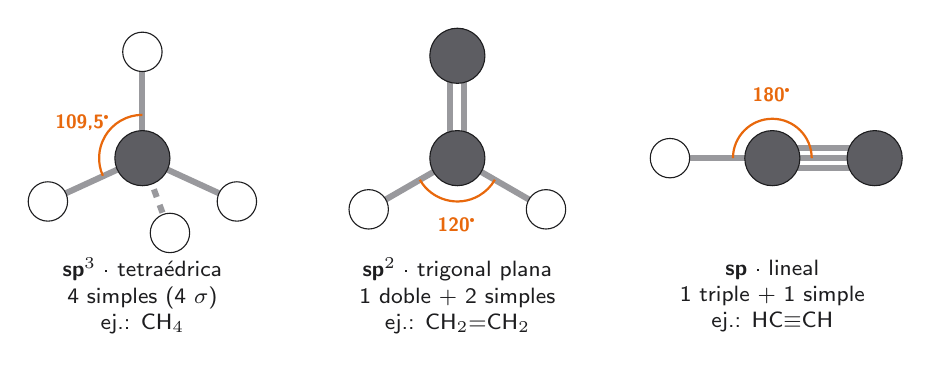
\begin{tikzpicture}
\tikzset{C/.style={circle,fill=gris!85!black,draw=tinta,minimum size=7mm,inner sep=0},
 H/.style={circle,fill=white,draw=tinta,minimum size=5mm,inner sep=0},
 st/.style={line width=2.2pt,gris!70}}
% tetraedrica
\begin{scope}
\coordinate (c) at (0,0);
\draw[st] (c)--(0,1.35); \draw[st] (c)--(-1.2,-0.55); \draw[st] (c)--(1.2,-0.55); \draw[st,dashed] (c)--(0.35,-0.95);
\node[H] at (0.35,-0.95) {}; \node[C] at (c) {}; \node[H] at (0,1.35) {}; \node[H] at (-1.2,-0.55) {}; \node[H] at (1.2,-0.55) {};
\draw[nar,thick] (0,0.55) arc (90:204:0.55); \node[nar,font=\scriptsize\bfseries] at (-0.75,0.45) {109,5°};
\node[pie] at (0,-1.75) {\textbf{sp$^3$} · tetraédrica\\4 simples (4 $\sigma$)\\ej.: CH$_4$};
\end{scope}
% trigonal plana
\begin{scope}[xshift=4cm]
\coordinate (c) at (0,0);
\draw[st] (-0.09,0)--(-0.09,1.3); \draw[st] (0.09,0)--(0.09,1.3);
\draw[st] (c)--(210:1.3); \draw[st] (c)--(330:1.3);
\node[C] at (c) {}; \node[C] at (0,1.3) {}; \node[H] at (210:1.3) {}; \node[H] at (330:1.3) {};
\draw[nar,thick] (210:0.55) arc (210:330:0.55); \node[nar,font=\scriptsize\bfseries] at (0,-0.85) {120°};
\node[pie] at (0,-1.75) {\textbf{sp$^2$} · trigonal plana\\1 doble + 2 simples\\ej.: CH$_2$=CH$_2$};
\end{scope}
% lineal
\begin{scope}[xshift=8cm]
\coordinate (c) at (0,0);
\draw[st] (c)--(-1.3,0); \draw[st] (0,0.13)--(1.3,0.13); \draw[st] (0,0)--(1.3,0); \draw[st] (0,-0.13)--(1.3,-0.13);
\node[H] at (-1.3,0) {}; \node[C] at (c) {}; \node[C] at (1.3,0) {};
\draw[nar,thick] (0.5,0) arc (0:180:0.5); \node[nar,font=\scriptsize\bfseries] at (0,0.8) {180°};
\node[pie] at (0,-1.75) {\textbf{sp} · lineal\\1 triple + 1 simple\\ej.: HC$\equiv$CH};
\end{scope}
\end{tikzpicture}}
\end{document}
